\documentclass[12pt]{article}

\usepackage{enumitem}
\usepackage[right=20mm, left=20mm]{geometry}
\usepackage{type1cm}
\usepackage{amssymb}
\usepackage[fleqn]{amsmath}
\usepackage{tikz}
\usepackage{multicol}
\usepackage{makecell}
\setlength{\columnsep}{1pt}
\usepackage{pgfplots}
\usepackage{float}
\usepackage{caption}
\usepackage{subcaption}
% \usepackage{subfig}
\usepackage{graphicx}

\usepackage{indentfirst}
\usepackage{lastpage}  
\usepackage{fancyhdr}
\pagestyle{fancy}

\usepackage[unicode=true,pdfusetitle,
 bookmarks=true,bookmarksnumbered=false,bookmarksopen=false,
 breaklinks=false,pdfborder={0 0 1},backref=false,colorlinks=false]
 {hyperref}

\makeatletter
\newenvironment{myalign*}{\ifvmode\else\hfil\null\linebreak\fi
  \hspace*{-\leftmargin}\minipage\textwidth
  \setlength{\abovedisplayskip}{0pt}%
  \setlength{\abovedisplayshortskip}{\abovedisplayskip}%
  \start@align\@ne\st@rredtrue\m@ne}%
{\endalign\endminipage\linebreak}

% Paper size
\topmargin -10mm
\textwidth 170mm
% \oddsidemargin -5mm
% \evensidemargin -5mm
\textheight 220mm

% Font setting
\usepackage{xeCJK}
% \setCJKmainfont{Noto Sans TC}
\setCJKmainfont{kaiu.ttf}


\renewcommand{\footnotesize}{\normalsize} 
\renewcommand{\headrulewidth}{0pt}
\renewcommand{\footrulewidth}{0pt}

\lhead{}
\chead{整合式線上教學平台ProgLearn}
\rhead{}

\lfoot{}
\cfoot{}
\rfoot{ 共 \pageref{LastPage} 頁 第  \thepage   頁} 

\makeatletter
\begin{document}
% \fontsize{14pt}{18pt}\selectfont
% \author{}
\date{}
\usetikzlibrary{automata, positioning, arrows}
% \maketitle
\tikzset{every state, accepting/.style={double distance=2pt}}
\captionsetup[figure]{labelfont={bf},name={圖},labelsep=period}

\noindent
\textbf{參賽隊名:} 普羅程式 \\
\textbf{作品名稱:} 整合式線上教學平台 ProgLearn

\begin{enumerate}
  \setlength{\parindent}{2em}
  \item 作品簡介
  \begin{enumerate}
    \setlength{\parindent}{2em}
    \item 創作動機與背景
    \par 在台灣,資訊科技領域受廣泛重視,且程式設計已被列為學校必修課程\cite{ref2}。
    儘管每年有數百萬學生修習程式課程\cite{ref3},但是在基層教育中卻存在許多問題。
    \item 作品目的
    \par 本計畫將建立一個名為 ProgLearn 的教學工具,專注於教師導向的教學工具,讓所有人都能做程式教學。
    \item 研究問題與專業領域
    \par 根據教師的教學需求,整理出四個主要問題:
    \begin{enumerate}[label=(\arabic*)]
      \setlength{\parindent}{2em}
      \item 教師的教學有諸多限制:
        \par 程式設計是實作很重要的課程,常見的線下教學方式需要使用廣播與管理系統,因為這些系統無法在授課時即時讓學生練習,導致老師不得暫停授課,給學生練習時間。
        這種情況可能使教師無法流暢教學,同時學生也難以吸收所學知識。
      \item 教師需要花多時間備課:
        \par 教師需要在上課前,準備線上課程的直播環境、準備課程教材、批改學生作業、上傳考題、課外時間回覆學生的各種問題等\cite{ref4}。
      \item 教師無法即時得知學生的狀況:
        \par 由於師生間缺乏互動的方式,讓學生難以保持學習熱忱,同時教師也無法即時注意學生的學習狀況,而影響教學成效\cite{ref7}。
      \item 教學工具零散:
        \par 在程式教學中,教師需要使用多種不同的工具和平台:準備教學教材的工具,如 PowerPoint 、 HackMD 等。準備課堂教學的環境,如 Google Meet 。以及繳交程式作業的系統,如 ITSA 程式自學平臺、TronClass 等。
        \par 由於這些軟體,並非針對教師的教學所設計,導致如批改、實作、設計教材、直播、上課,仍需要透過其他軟體或平台來實現。缺乏整合的教學工具,不但增加了環境的建置難度,也提高教師的教學負擔。
    \end{enumerate}
    \par 基於以上問題,本系統跨足教育領域,通過改進教師的教學方式,幫助教師以最小的成本實現預期的教學效果,從而提高學生的學習體驗和效果。
    \item 創新創意
      \par 本系統為符合教師的教學需求,設計出以下幾種創新功能:
      \begin{enumerate}[label=(\arabic*)]
        \setlength{\parindent}{2em}
        \item 課堂直播
          \begin{itemize}
            \item 即時同步的投影片:此直播實際上是一個投影片,可以將老師對投影片的繪畫、換頁等操作同步到學生的畫面中。
            \item 可隨時切換的投影片:讓學生在直播期間,可以按照自己的學習速度切換到其他簡報,提供學生學習的彈性。
          \end{itemize}
        \item 互動式講義
          \begin{itemize}
            \item 滾動式講義:透過 Markdown 呈現課程講義,讓學生更方便地查看課程講義,也加快教師編寫教材的速度。
            \item 跟隨模式:課程直播時,在學生的頁面中會以淺黃色提示老師正在教學的內容。
            \item 嵌入式的程式問題:讓學生能在講義區直接作答,並且能即時得知答案是否正確,教師也可以隨時得到學生的答題狀態。
          \end{itemize}
        \item 學生的回看功能
          \begin{itemize}
            \item 學生在直播中,可以任意切斷到其他投影片,並隨時能切換到老師目前的進度。
            \item 學生在課後,可以再次觀看過往的上課直播,當學生切換到其他投影片時,時間軸會自動暫停。播放時,可以讓學生回到上次的進度。
          \end{itemize}
        %\par 使用情境:演算法課程中,老師剛上完搜尋演算法並出了一個習題,此習題是搜尋程式碼的片段並挖了幾個空格,學生填答空格後,老師能即時取得學生的填答狀況。(同步回答圖)
      \end{enumerate}
    \item 主要功能
    \par 該系統提供課堂教學系統和課後作業系統。
    課堂教學系統提供投影片直播、投影片繪畫、互動式講義、學生的答題統計的功能。
    課後作業系統提供自動批改程式碼作業的功能。
    \item 實用性與預期貢獻
    \par 協助教師提高教學效率,並且提高學生的學習效果。在未來能將此系統提供給如學校、補習班、講座等老師使用。
  \end{enumerate}

  \item 需求分析
    \par 本計畫將依循軟體工程流程與方法進行需求擷取與分析、架構與介面設計。
    \begin{enumerate}
      \setlength{\parindent}{2em}
      \item 功能性需求:%以itemindent調整縮排,但應該有更好的做法能一同縮排。
        \begin{enumerate}[itemindent=12pt]
          \item [A.] 班級與課程功能
            \begin{enumerate}[itemindent=24pt]
              \item [A-1.] 教師可新增與查詢自己的課程,並於特定課程中新增章節。
              \item [A-2.] 教師可於特定章節中查看此章節中,學生的答題統計、問答紀錄。
            \end{enumerate}
          \item [B.] 直播投影片功能
            \begin{enumerate}[itemindent=24pt]
              \item [B-1.] 教師可於特定章節中上傳課程投影片。
              \item [B-2.] 教師可於教學頁面中直播模式,使學生的投影區畫面與教師相同。
              \item [B-3.] 教師可於教學頁面中
              \item [B-4.] 學生可於教學頁面中觀看此章節的投影片。
            \end{enumerate}
          \item [C.] 講義功能
            \begin{enumerate}[itemindent=24pt]
              \item [C-1.] 教師可編輯章節的講義,並於講義中新增與編輯文字、圖形與互動式元件。
              \item [C-2.] 教師可開啟黑板模式,讓特定學生能在投影片中繪圖寫字。
              \item [C-3.] 學生可於教學頁面中觀看此章節的投影片,並與互動性元件互動,如勾選方框、按下按鈕等。
            \end{enumerate}
          \item [D.] 答題功能
            \begin{enumerate}[itemindent=24pt]
              \item [D-1.] 教師可於特定章節中新增題目,並且可以在現有題目系統(如: AtCoder%$\footnote{https://atcoder.jp/}$
              )直接抓取題目。
              \item [D-2.] 教師可於特定章節中查看各學生於特定作業的答題情況,內容包含繳交的程式碼與分數。
              \item [D-3.] 教師可針對答題情況,留下教師建議。
              \item [D-4.] 學生可於特定章節中查看並解決此章節的課後練習題目。
            \end{enumerate}
          \item [E.] 教學頁面功能
            \begin{enumerate}[itemindent=24pt, label=E-\arabic*.]
              \item 學生可於投影片區觀看並操作投影片。
              \item 學生可於程式區編輯 JS 程式碼,並且能執行與查看結果。
              \item 教師可查看各學生執行的程式碼與結果。
              \item 教師可控制黑板模式並使用互動性功能。
            \end{enumerate}
          \end{enumerate}
      \item 非功能性需求
        \begin{enumerate}[itemindent=12pt]
          \item [A.] 使用者介面與人為因素
          \begin{enumerate}[itemindent=24pt]
            \item [A-1.] 使用者:程式設計課程的老師、學生
            \item [A-2.] 使用者的介面設計:簡單並且易上手、高度的功能整合、即時獲得使用者的反饋與資訊。
            \item [A-3.] 使用者的引導與教學:直觀的UI設計並且對所有老師做系統的使用培訓。
          \end{enumerate}
          \item [B.] 硬體
            \begin{enumerate}[itemindent=24pt]
              \item [B-1.] 使用者的使用設備:使用設備以電腦為主、手持設備為輔,並針對電腦使用最佳化。
              \item [B-2.] 使用者的設備限制:所有能瀏覽網頁的設備皆可使用。
            \end{enumerate}
          \item [C.] 效能
            \begin{enumerate}[itemindent=24pt]
              \item [C-1.] 反應時間:同一課程能讓100人同時使用,並在0.5秒內回應使用者,以保障使用者的上課體驗。
              \item [C-2.] 容量限制:限制每位教師在單一章節中,只能上傳20MB以下的投影片。
              \item [C-3.] 課堂限制:每位教師的課程需要經過管理員審核後才能開課,並且每位教師以開設5門課為限。
              \item [C-4.] 課堂人數:同一課程最多只能有100位學生。
            \end{enumerate}      
          \item [D.]錯誤處理:
            \begin{enumerate}[itemindent=24pt]
              \item [D-1.] 系統遇到不正常的負載:針對大量請求的用戶限制封包的流量。
              \item [D-2.] 系統遇到高負載:使用排隊來限制同時登入人數。
            \end{enumerate}
        \end{enumerate}
      \item 系統設計
      \par 本系統是架設於網路上的 Web 應用系統,以下將針對系統的設計分為系統架構、系統介面說明:
        \begin{enumerate}[label=(\arabic*)]
        \setlength{\parindent}{2em}
          \item 系統架構
          \par 根據需求擷取與分析所述,系統架構如圖\ref{arc1}所示,
          在 Proglearn 系統內(如圖\ref{arc1}),
          包括前端服務器(Web Application Server、Single Page Application)、
          主要後端服務器(Business Backend)、
          課程管理服務器(Course Manage Server)、
          線上解題服務器(Online Judge Server)、
          資料庫(Database)等容器。
          \begin{figure}[htb]
            \centering
            \begin{subfigure}{0.45\linewidth}
              \centering
              \href{https://raw.githubusercontent.com/programingtw/proglearn-plan/main/img/arc1.jpg}{
                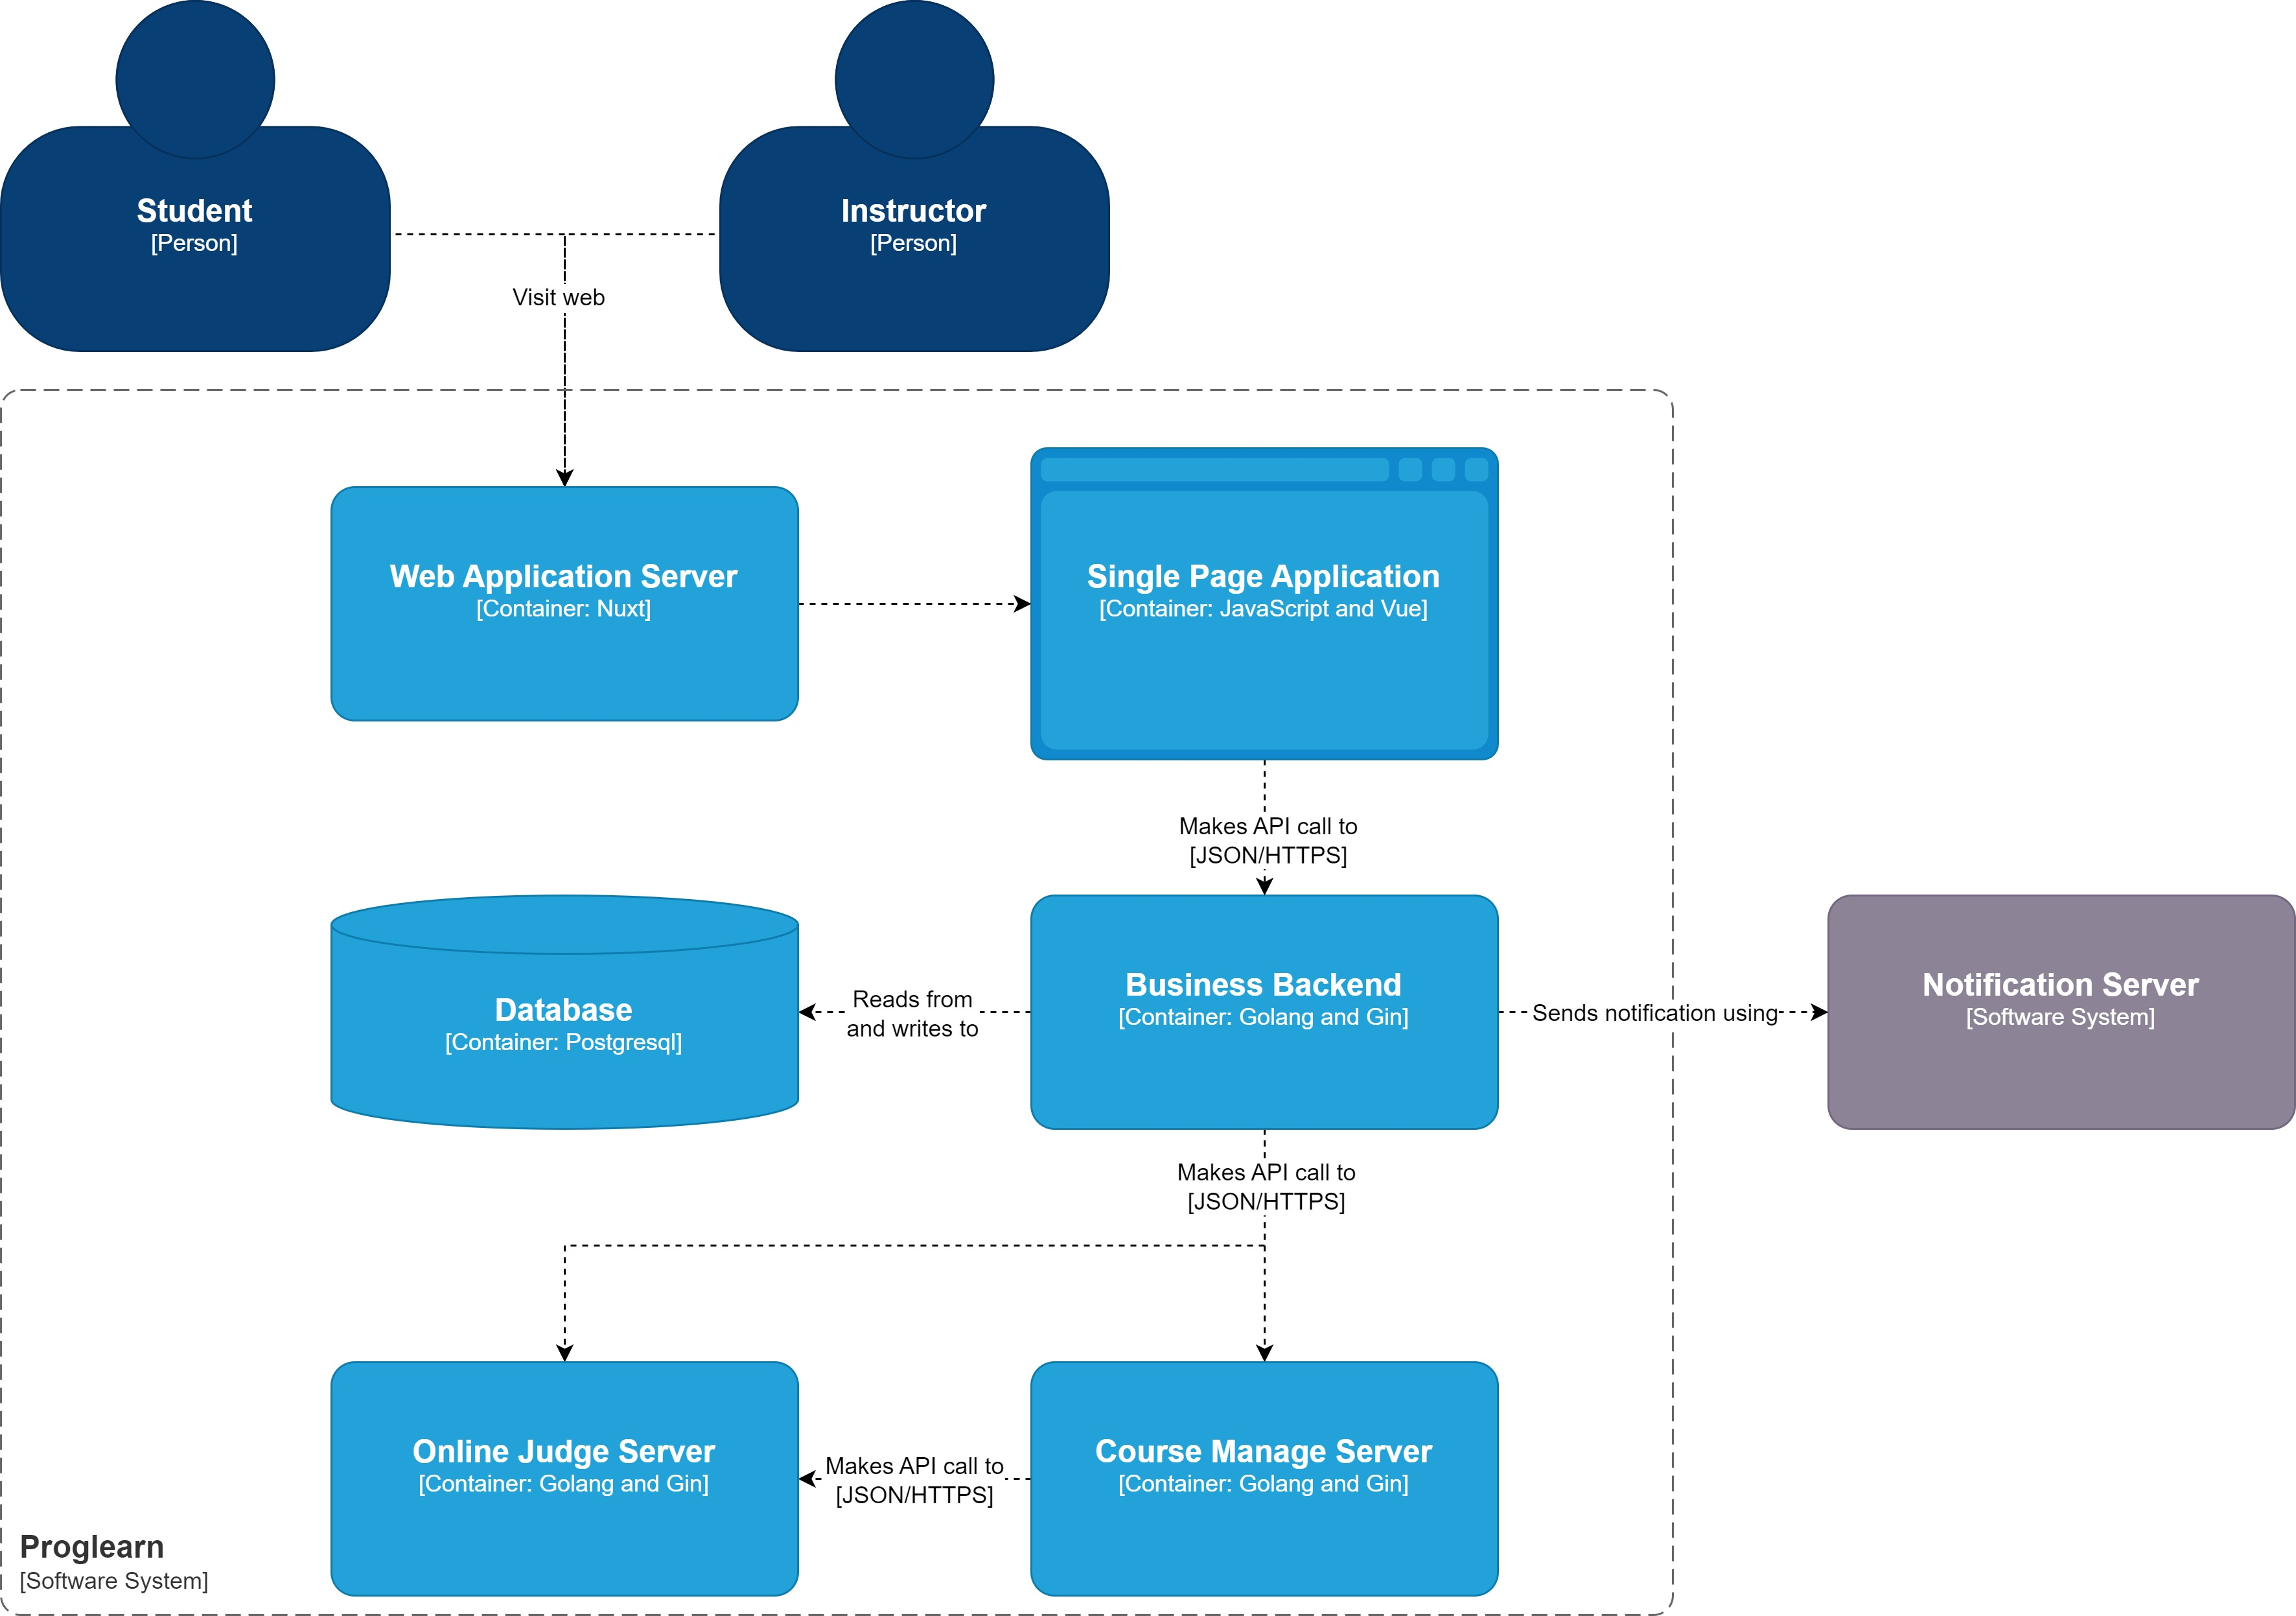
\includegraphics[width=0.65\textwidth]{./img/arc1.jpg}
              }
              \caption{Proglearn 系統架構}
              \label{arc1}            
            \end{subfigure}
            \begin{subfigure}{0.45\linewidth}
              \centering
              \href{https://raw.githubusercontent.com/programingtw/proglearn-plan/main/img/arc2.jpg}{
                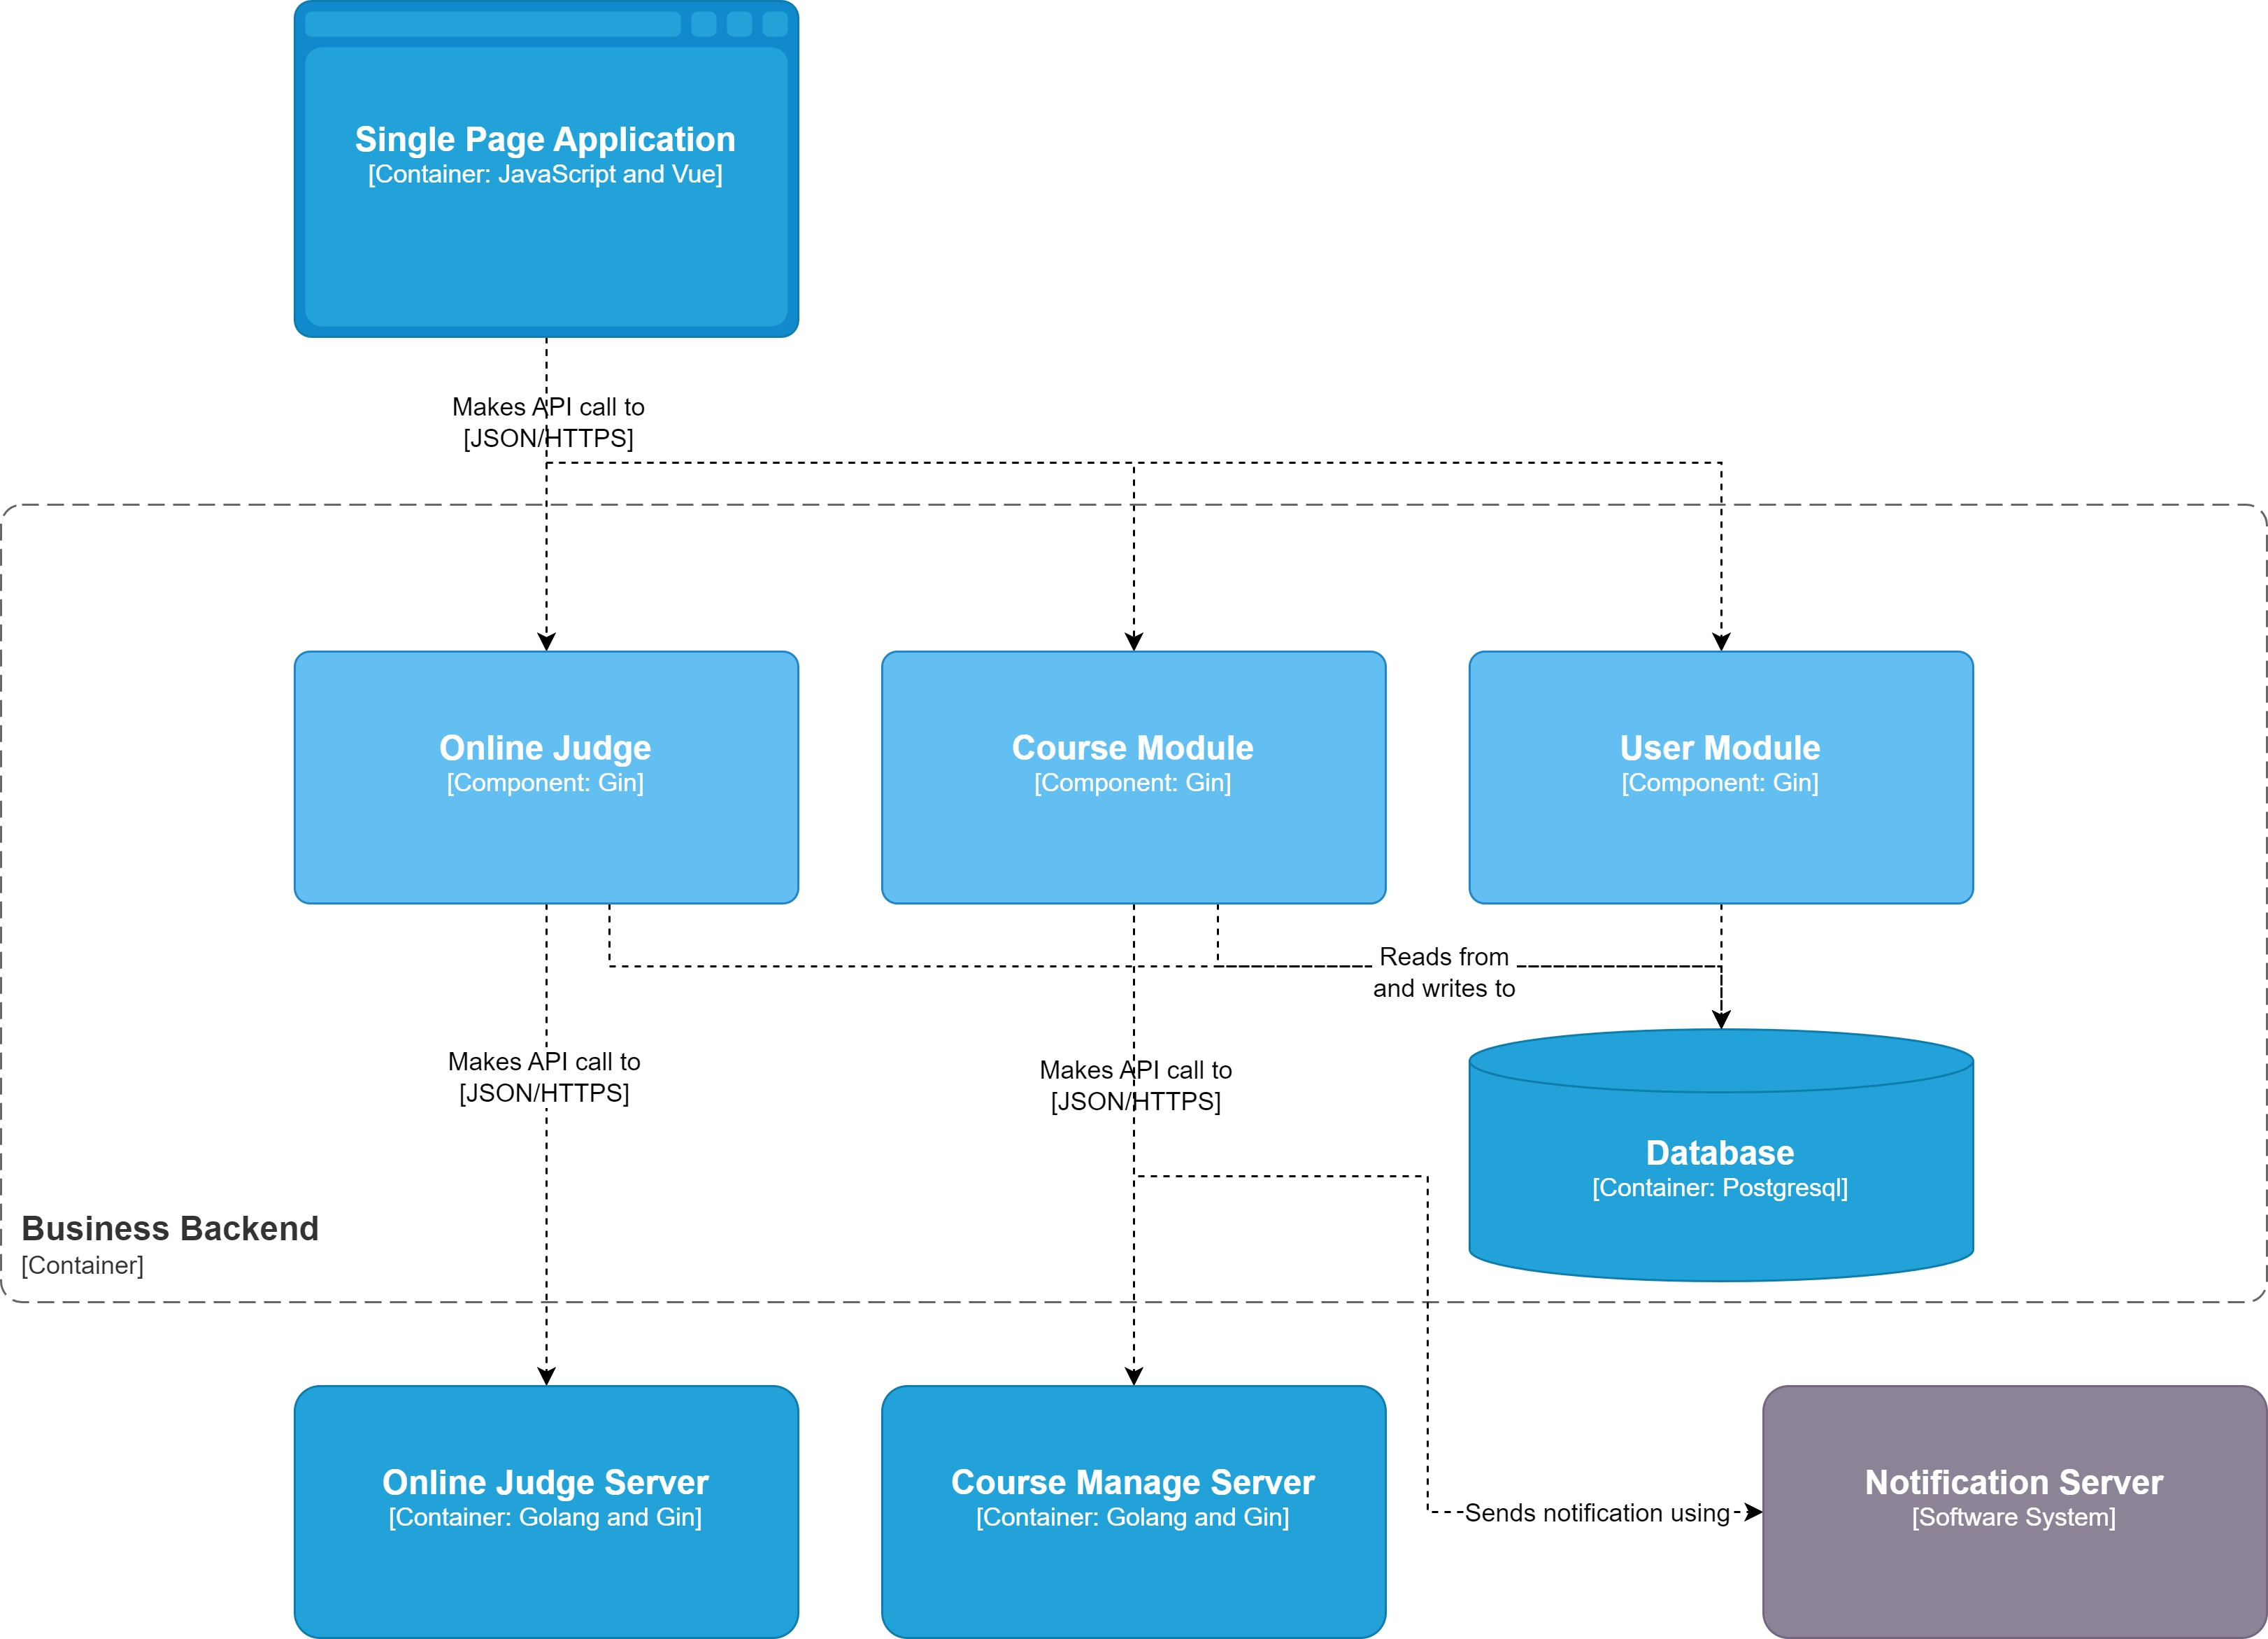
\includegraphics[width=0.65\textwidth]{./img/arc2.jpg}
              }
              \caption{主要後端服務器架構}
              \label{arc2}
            \end{subfigure}
            \bigskip
            \begin{subfigure}{0.45\linewidth}
              \centering
              \href{https://raw.githubusercontent.com/programingtw/proglearn-plan/main/img/arc3.jpg}{
                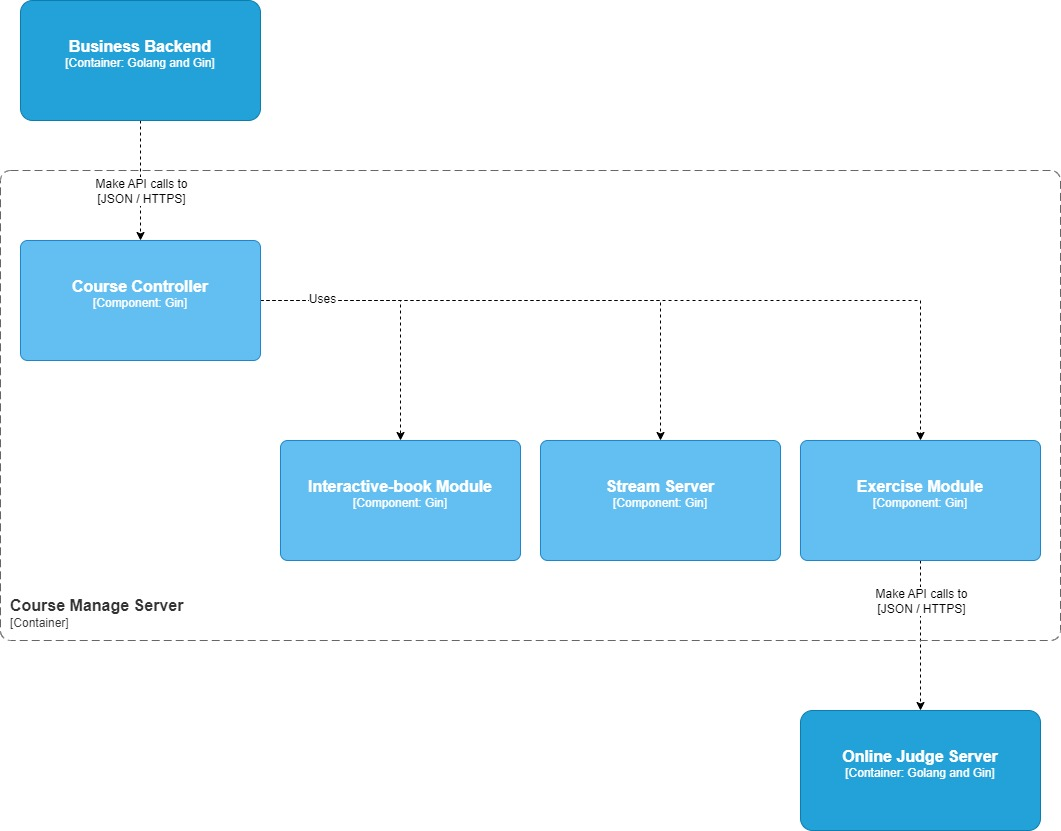
\includegraphics[width=0.65\textwidth]{./img/arc3.jpg}
              }
              \caption{課程管理服務器架構}
              \label{arc3}
            \end{subfigure}
            \begin{subfigure}{0.45\linewidth}
              \centering
              \href{https://raw.githubusercontent.com/programingtw/proglearn-plan/main/img/arc4.jpg}{
                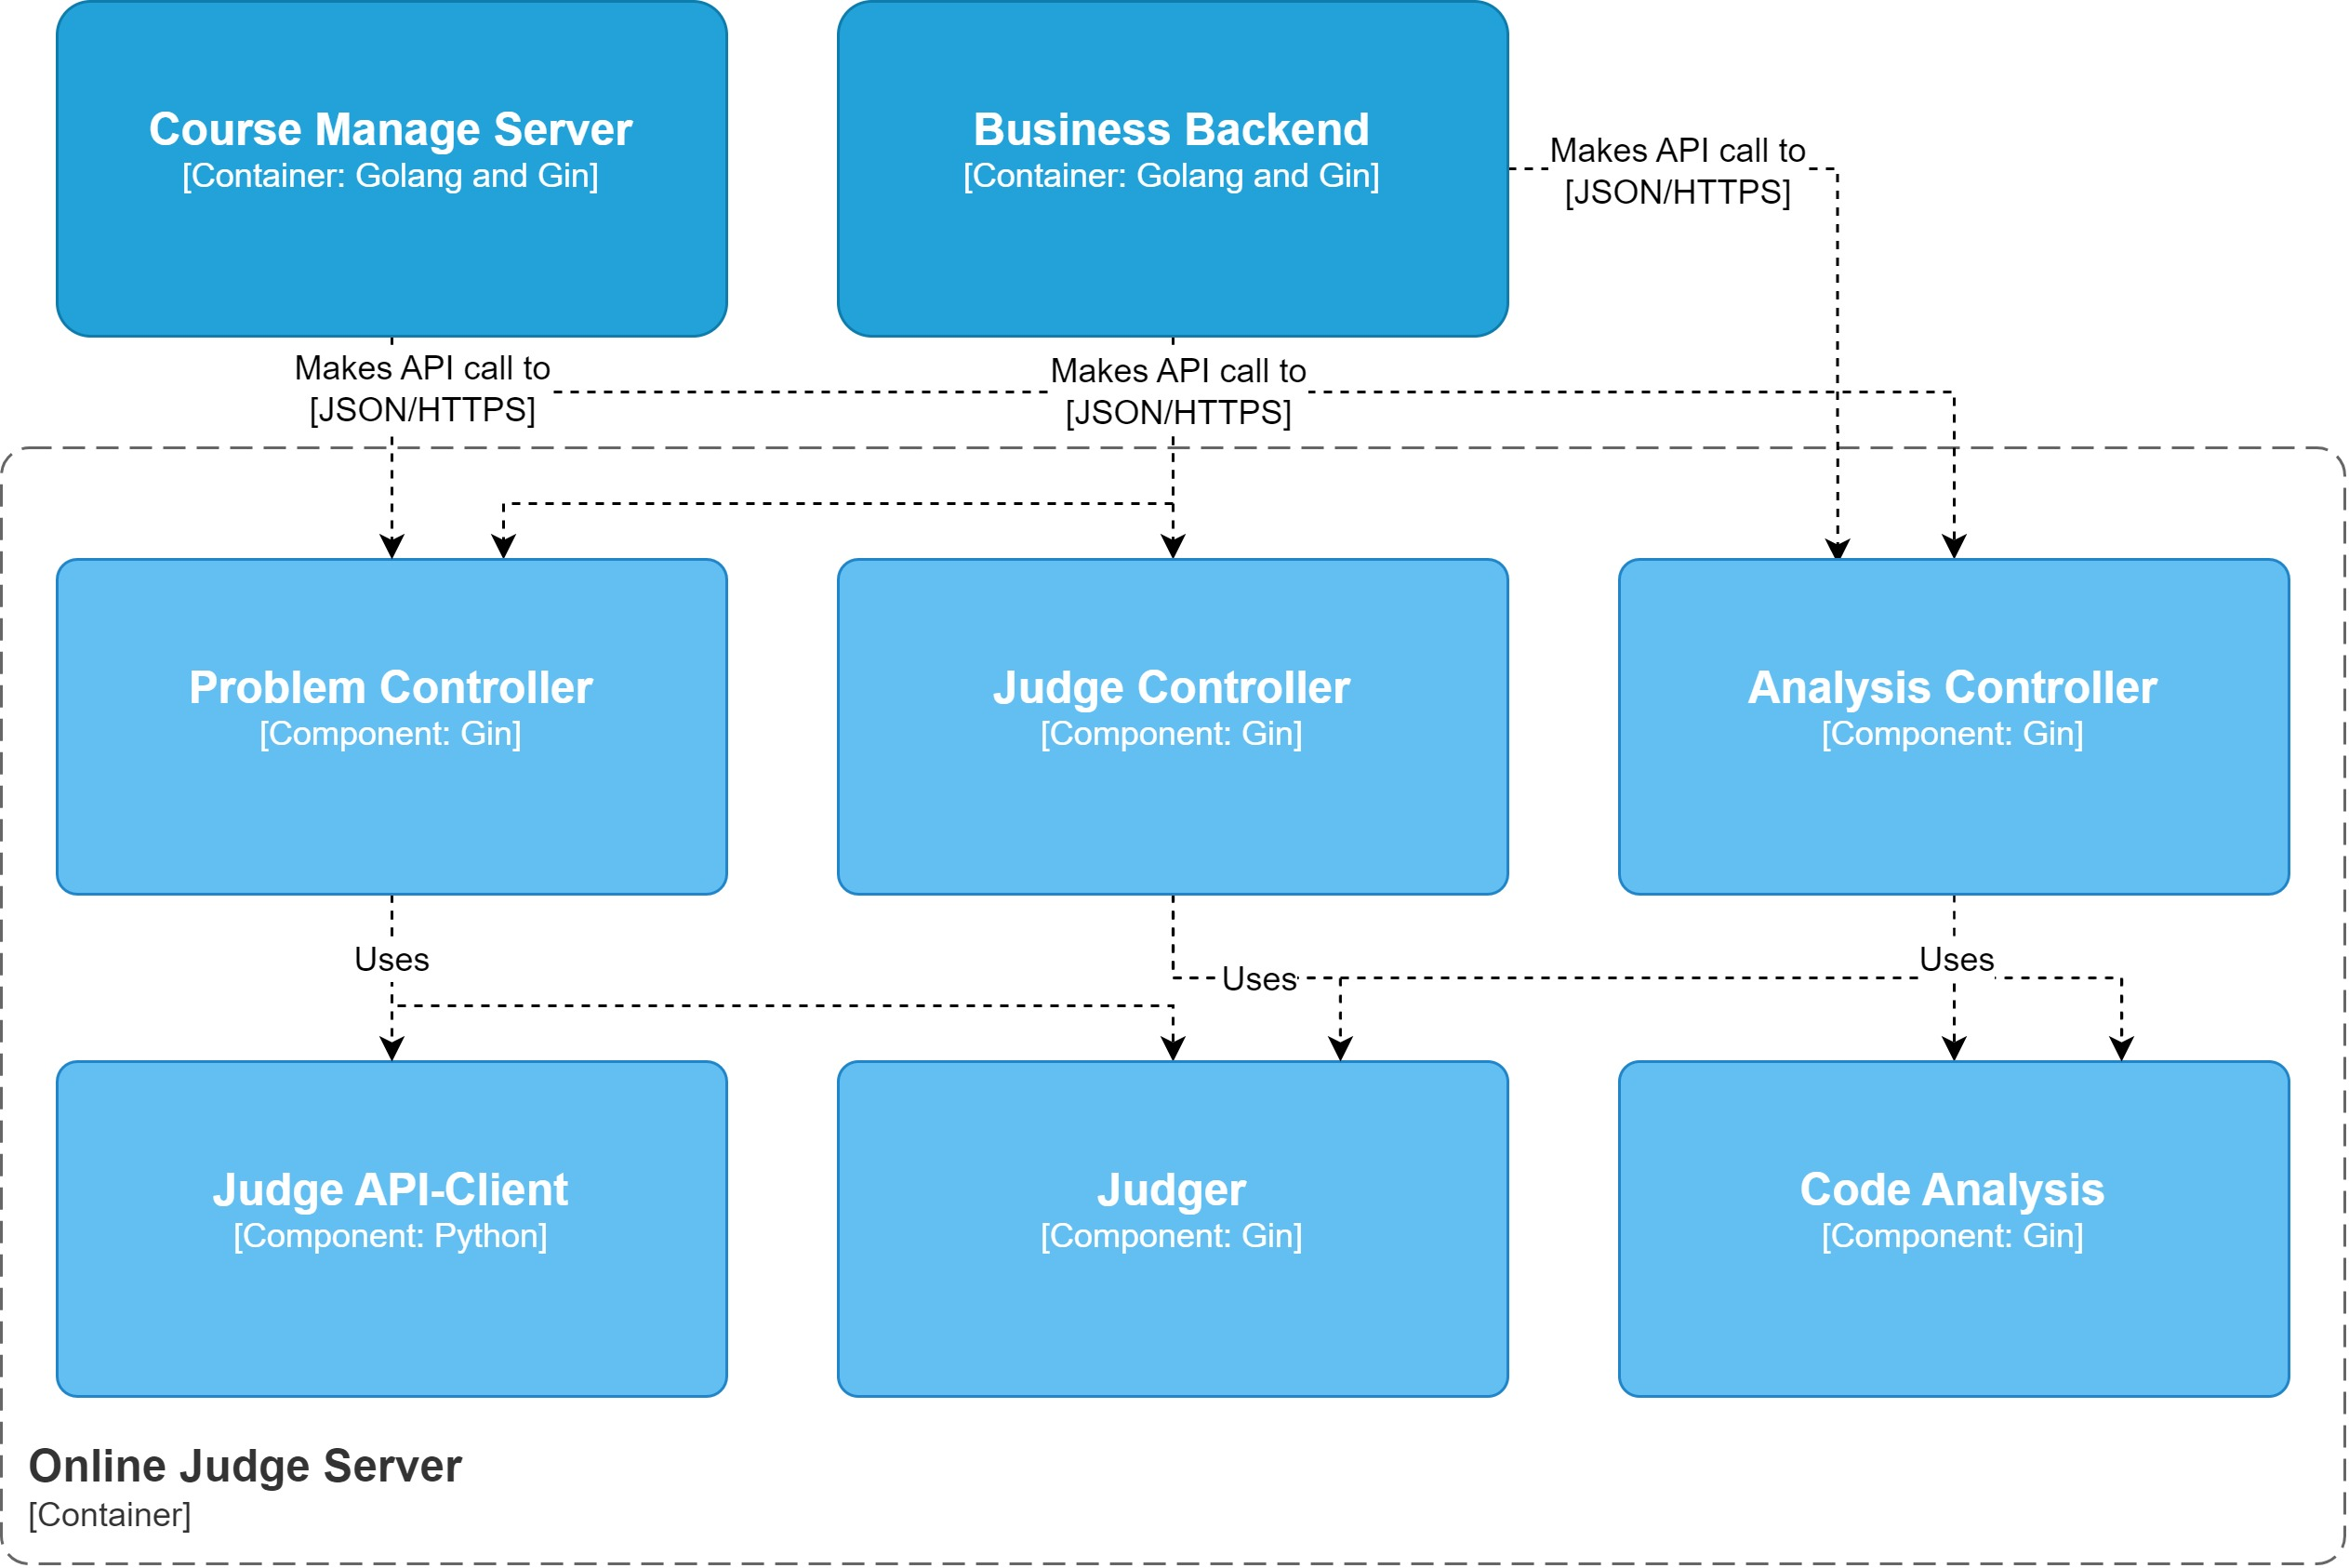
\includegraphics[width=0.65\textwidth]{./img/arc4.jpg}
              }
              \caption{線上解題服務器架構}
              \label{arc4}            
            \end{subfigure}
            \caption{系統架構設計 (點擊可看大圖)}
          \end{figure}
      
          \par 主要後端服務器(如圖\ref{arc2})
            負責處理與管理使用者資料(User Module)、課程模組(Course Module)、題目模組(Online Judge)。
          
          \par 課程管理服務器(如圖\ref{arc3})
            包括影音服務器(Video Server)、投影片模組(Code-Slides Module)、練習模組(Exercise Module)。
            投影片模組將使用 CodeMirror 作為編輯器,並且提供使用 JavaScript 程式碼撰寫投影片。
            前端呈現如圖\ref{arc5},學生能夠同時看到教師的畫面及投影片。
            % 接著使用
          \begin{figure}[H]
            \centering
            \href{https://raw.githubusercontent.com/programingtw/proglearn-plan/main/img/testboard.png}{ 
              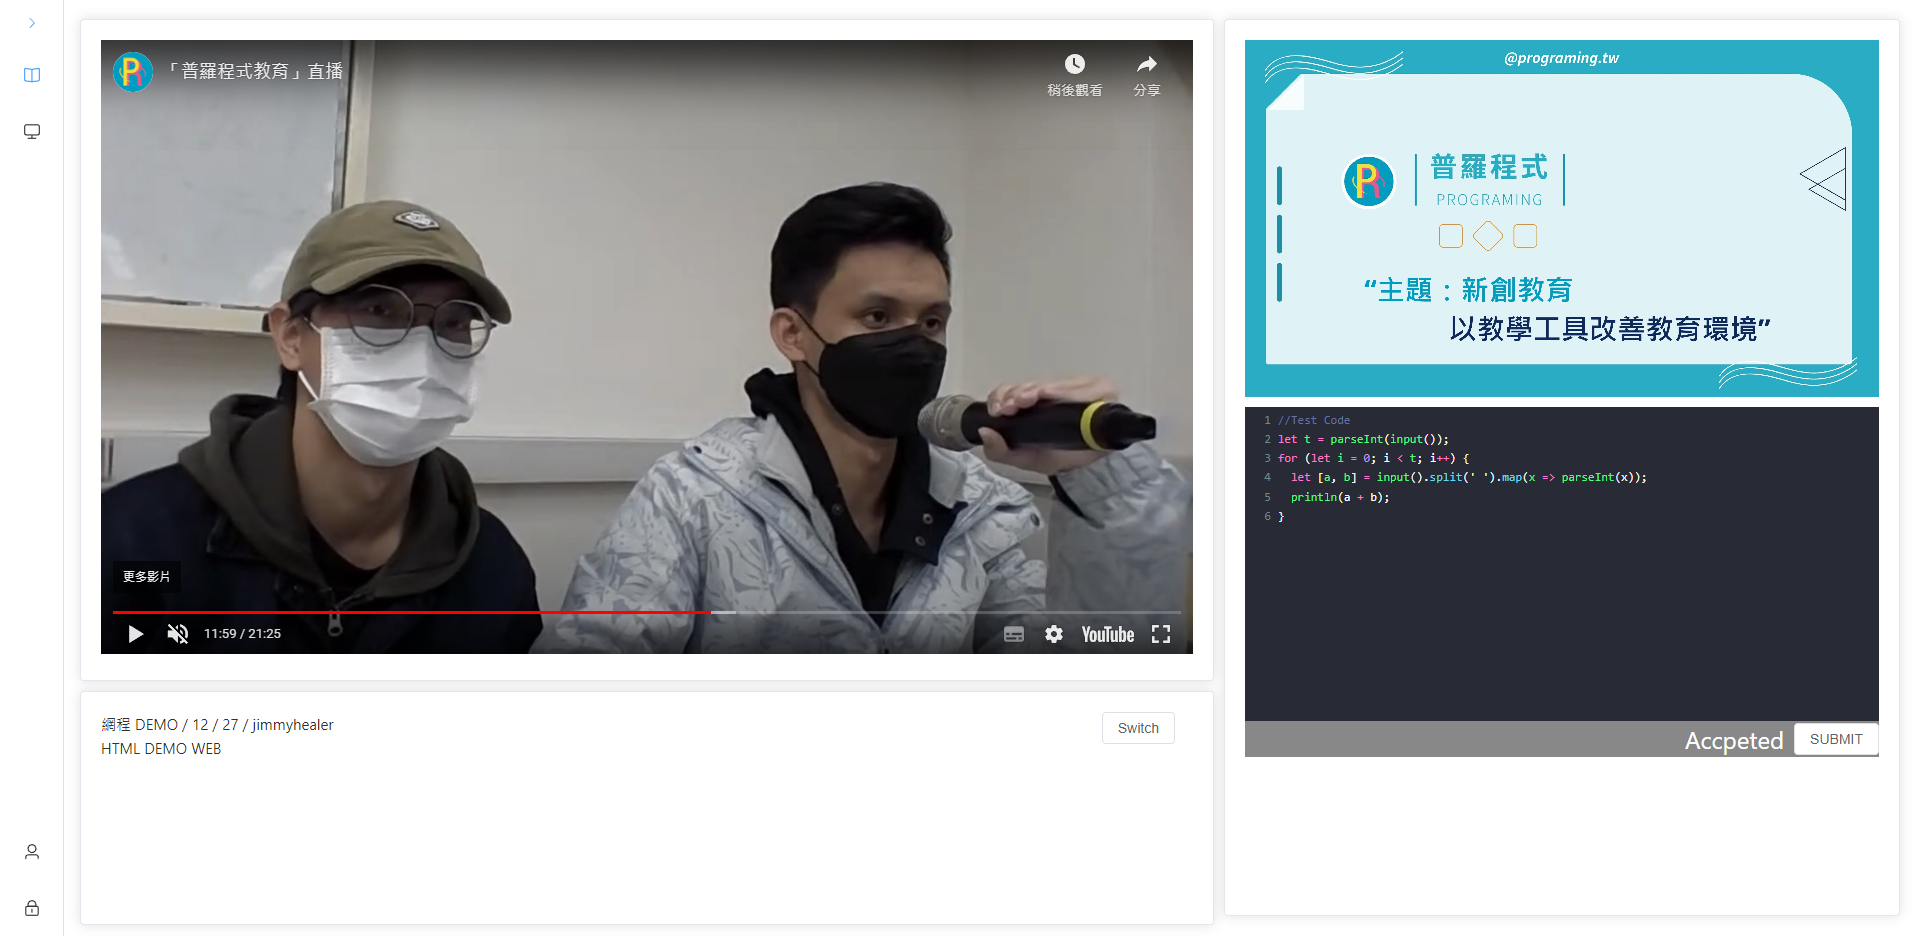
\includegraphics[width=0.5\textwidth]{./img/testboard.png}
            }
            \caption{前端教學頁面示意圖 (點擊可看大圖)}
            \label{arc5}
          \end{figure}
          \par 線上解題服務器(如圖\ref{arc4})
            包括線上題目抓取模組(Judge API-Client)、程式碼批改模組(Judger)、程式碼分析模組(Code Analysis)。
             Judge API-Client 是使用開源專案 api-client \cite{apiclient} 作為線上題目抓取模組,方便教師可以使用現有的題目做修改。
             Judger 是參考開源專案 go-judge \cite{judger1} 、JudgeServer \cite{judger2} 開發出沙盒程式碼執行環境及程式碼批改模組。
             Code Analysis 將採用多標籤辨識模型實現,後續章節將針對此核心技術進行更詳細的說明。
        
          \item 系統介面設計
            \par 系統的使用頁面主要為課堂教學頁面。並針對不同的使用者,設計兩種使用介面:
            \begin{itemize}
              \item 教師:能夠管理投影區與互動區,並取得學生的答題狀況。
              \item 學生:能夠觀看投影片、互動區的內容,互動區包含滾拉式的 Markdown 講義,並且嵌入以程式為主的互動性問題,讓學生作答。
            \end{itemize}
          \end{enumerate}  
    \end{enumerate}
  \item 開發技術介紹
    \begin{enumerate}[label=(\arabic*)]
      \setlength{\parindent}{2em}
      \item 程式語言:TypeScript, Golang
      \item 前端設計:Vue3, Element Plus, chart.js, Codemirror, Vue Router, Pinia   
      \item 後端設計:Gin, Websocket, WebRTC
      \item 資料庫:PostgreSQL
      \item 開發工具:Git, Docker, VSCode, Postman
    \end{enumerate}
  
  \item 作品展示
    \begin{figure}[H]
      \centering
      \href{https://raw.githubusercontent.com/programingtw/proglearn-plan/main/img/list.png}{ 
        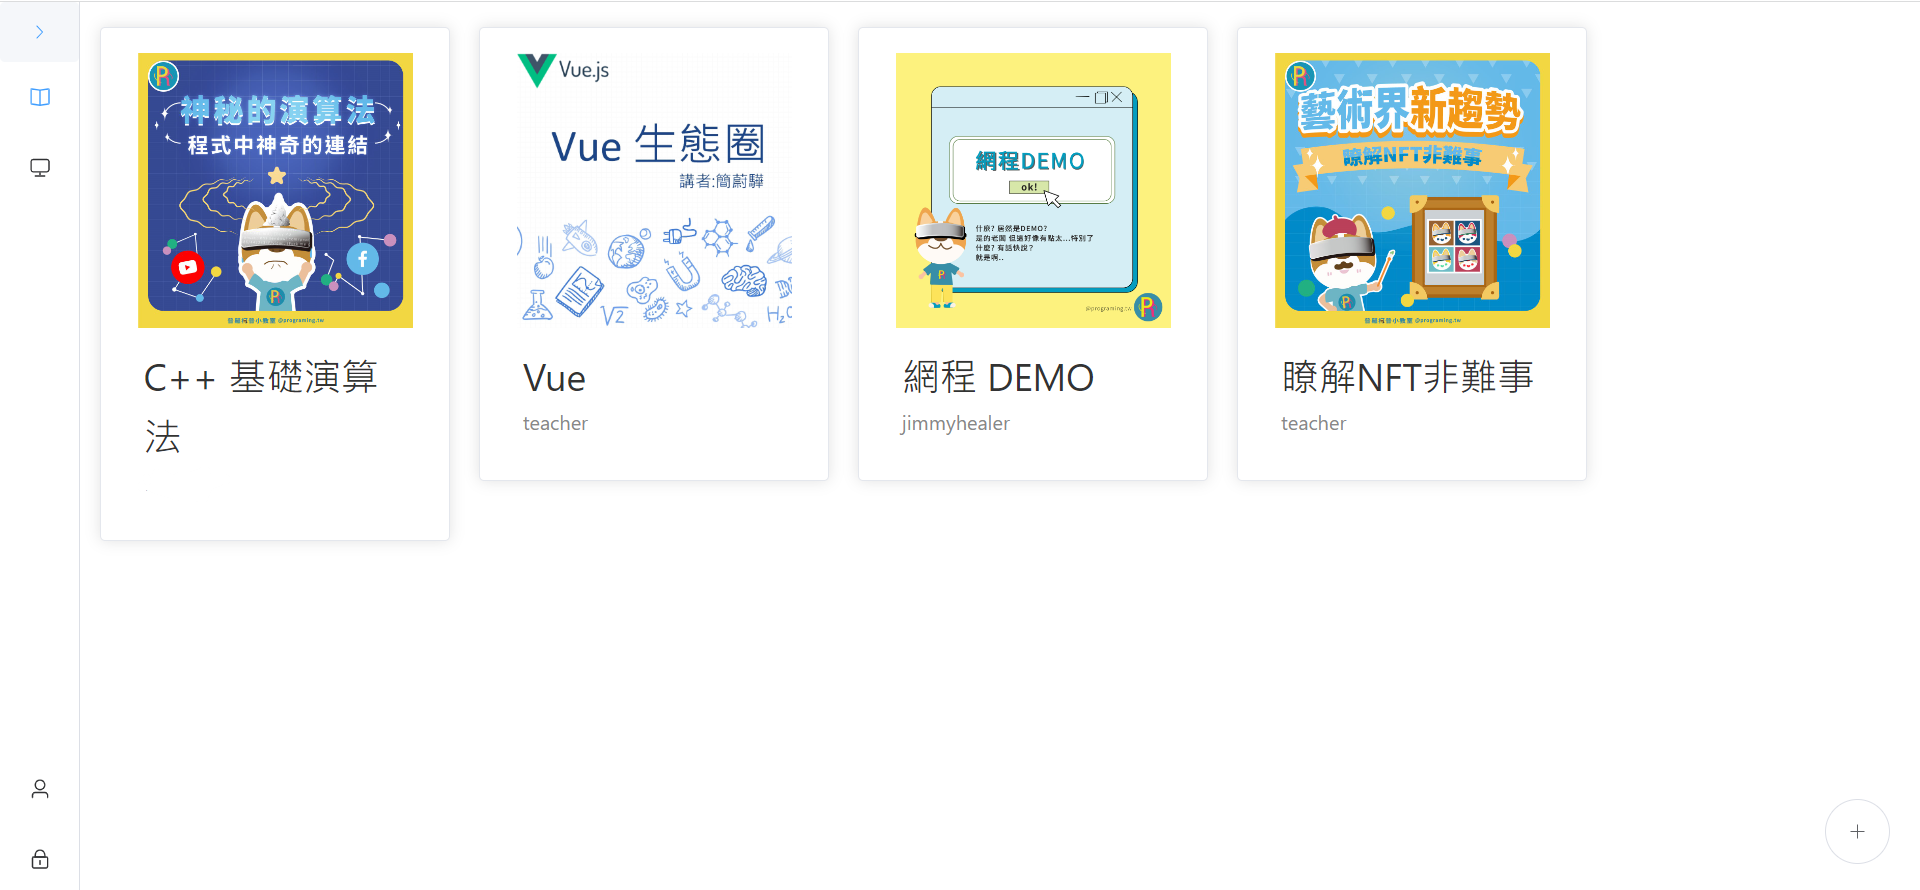
\includegraphics[width=0.5\textwidth]{./img/list.png}
      }
      \caption{課程清單頁面 (點擊可看大圖)}
      \label{arc6}
    \end{figure}

    \begin{figure}[H]
      \centering
      \href{https://raw.githubusercontent.com/programingtw/proglearn-plan/main/img/course.png}{ 
        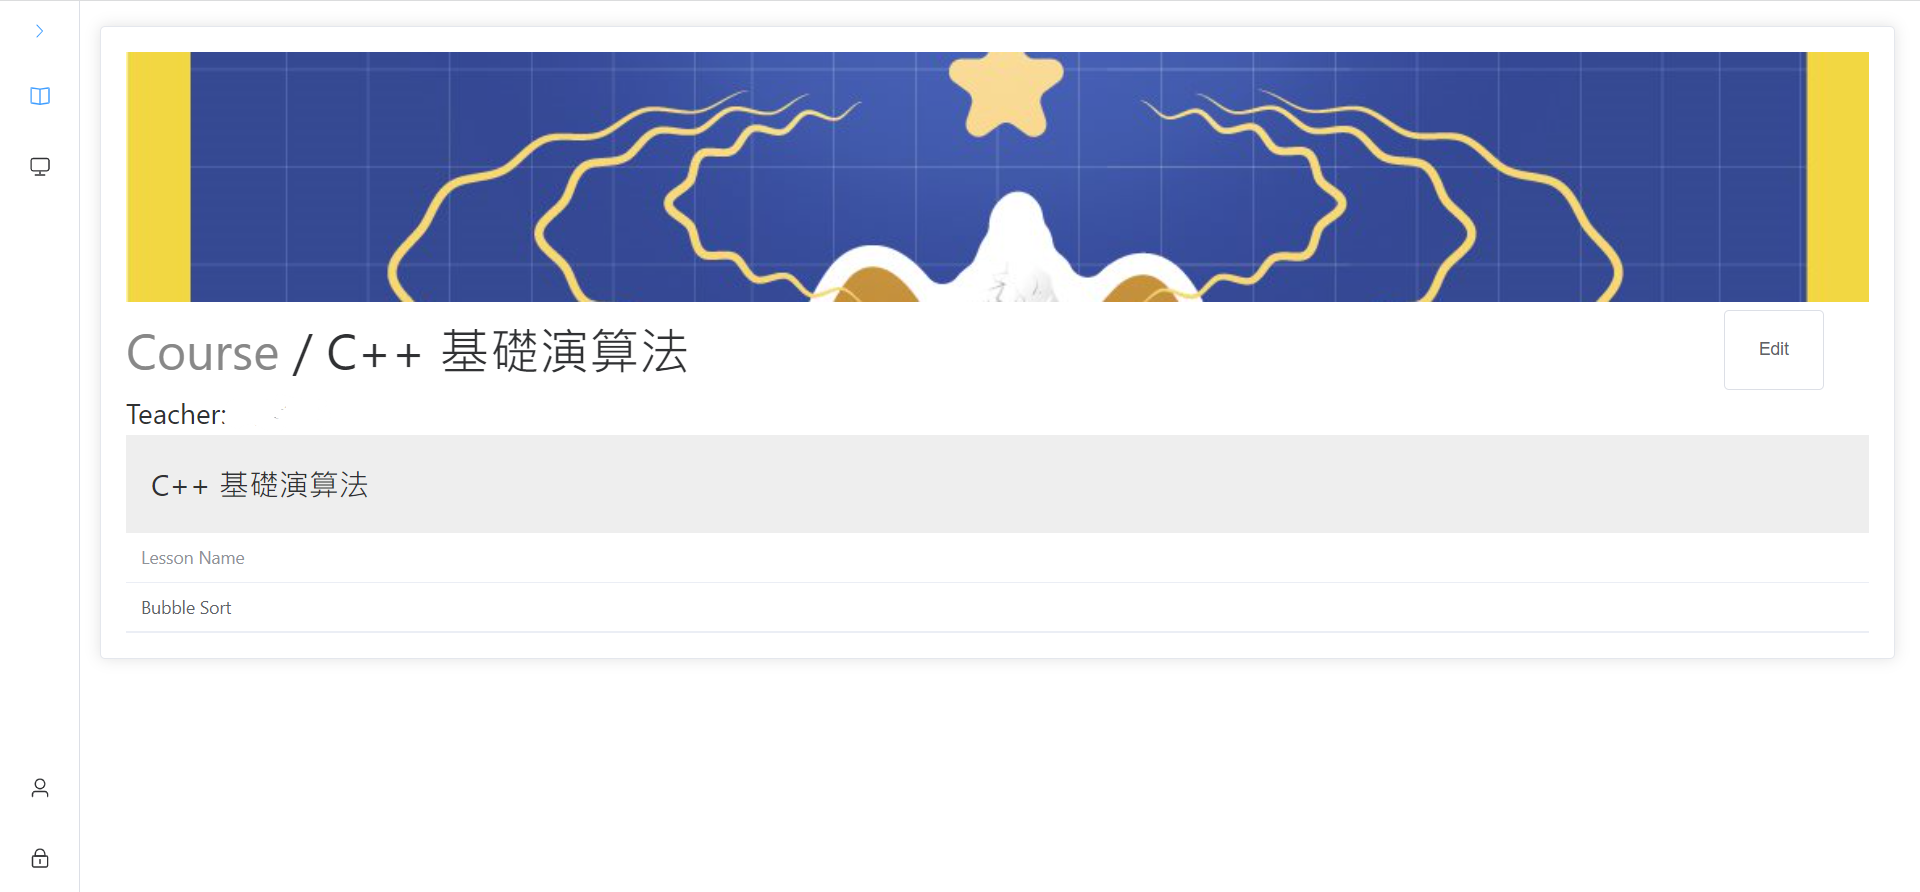
\includegraphics[width=0.5\textwidth]{./img/course.png}
      }
      \caption{課程資訊頁面 (點擊可看大圖)}
      \label{arc7}
    \end{figure}

    \begin{figure}[H]
      \centering
      \href{https://raw.githubusercontent.com/programingtw/proglearn-plan/main/img/testcode.png}{ 
        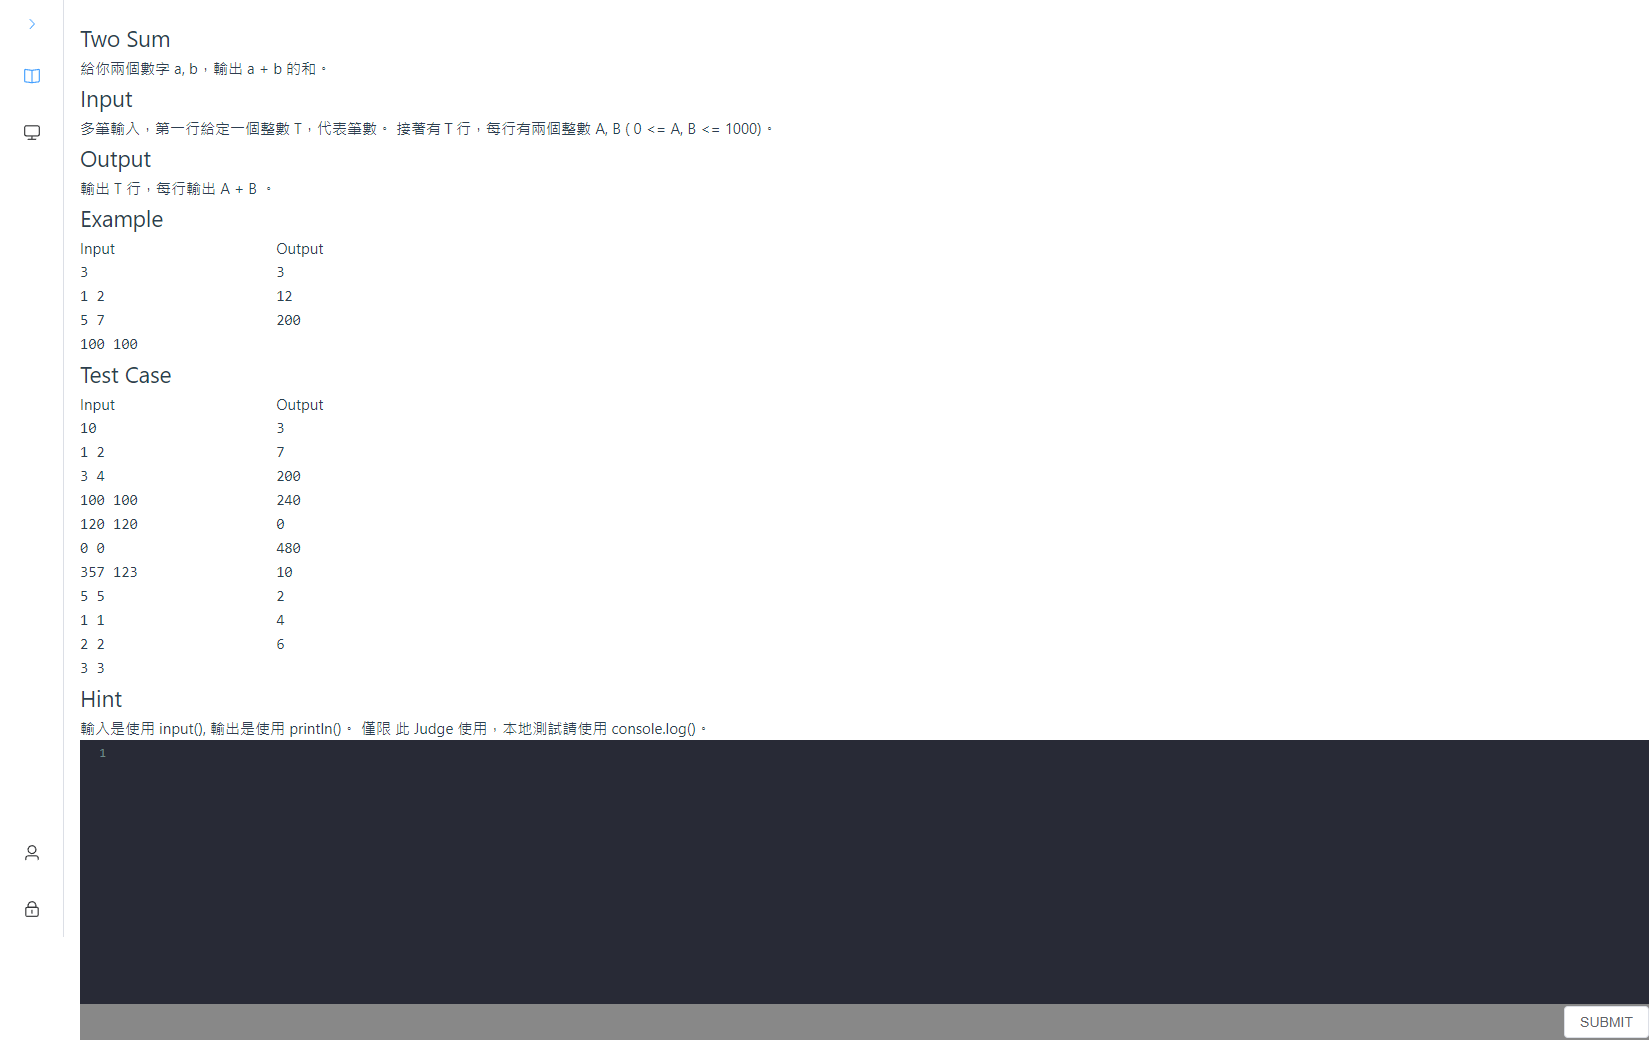
\includegraphics[width=0.5\textwidth]{./img/testcode.png}
      }
      \caption{課程作業頁面 (點擊可看大圖)}
      \label{arc8}
    \end{figure}

    \begin{figure}[H]
      \centering
      \href{https://raw.githubusercontent.com/programingtw/proglearn-plan/main/img/feedback.png}{ 
        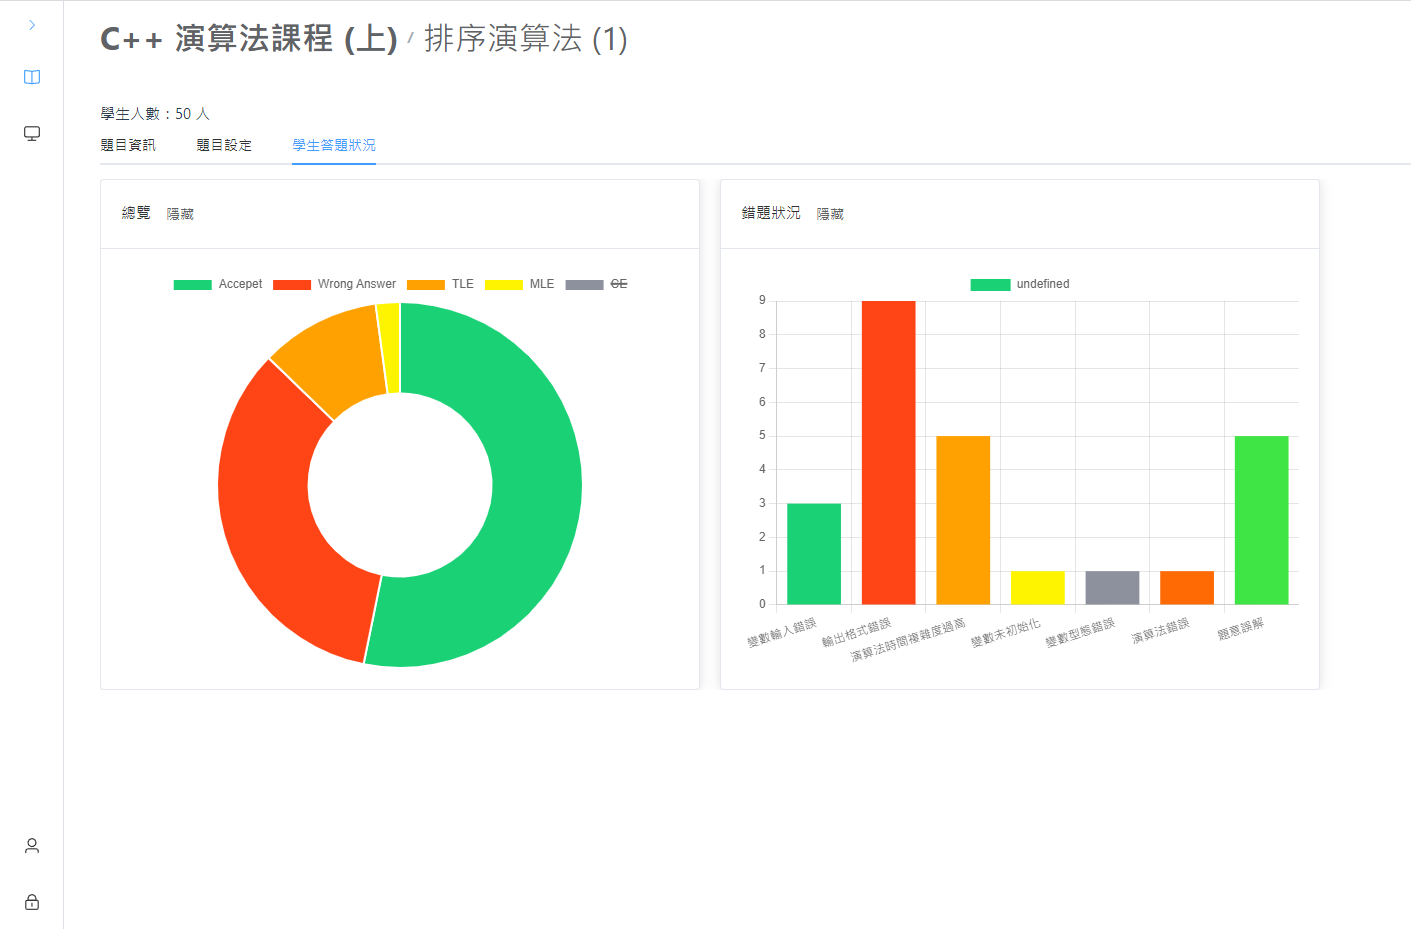
\includegraphics[width=0.5\textwidth]{./img/feedback.png}
      }
      \caption{課程作業回饋 (點擊可看大圖)}
      \label{arc9}
    \end{figure}

  \item 未來與展望
    \par 未來將增加與改善以下四種功能:
    \begin{enumerate}
      \item 增加自動回饋系統,讓教師可以快速了解學生的學習進度和弱點,減少教師在教學與備課的工作量。
      \item 增加智能助教系統,自動批改學生作業並提出建議,讓教師能夠快速掌握學生的學習狀況。
      \item 增加互動式講義的功能,讓教師與學生之間有更多互動,將抽象的概念視覺化,讓學生更容易理解並加深印象。
      \item 增加教材的輔助 AI,能夠根據教師的教學內容,提供文字補全與編寫建議,以提高教師編寫教材的效率。
    \end{enumerate}
    \par 並且以創業與經營為目標,提供教學系統服務給程式教育的教師,

  \item 參考文獻
    \renewcommand{\section}[2]{}
    \begin{thebibliography}{99}
      \bibitem{ref2} 十二年國民基本教育課程綱要。民112年2月14日,取自:https://www.naer.edu.tw/PageSyllabus?fid=52。
      \bibitem{ref3} 政府資料公開平台(民111年6月29日)。全臺灣各級學校之學生數及畢業生數資料。民112年2月14日,取自:https://data.gov.tw/dataset/31436。
      %\bibitem{ref5} 聯合新聞網(民110年3月8日)。中小學資訊教師荒! 多校找自然師兼任遭批不專業。民112年2月14日,取自:https://udn.com/news/story/6885/5303319。
      \bibitem{ref4} 張瑞賓、李建華。"遠距教學常態化問題之探討與建議。" 臺灣教育評論月刊 10.6 (2021): 27-34。
      \bibitem{ref7} 岳修平、梁朝雲。 "綜整學生,教師與教學情境考量的遠距教學預測模型。" 教育資料與圖書館學 52.1 (2015): 33-57+。
      %\bibitem{ref8} De Giusti, Armando. "Book review: Policy brief: Education during COVID-19 and beyond." Revista Iberoamericana de Tecnología En Educación y Educación En Tecnología 26 (2020): 110-111.
      %\bibitem{ref9} Tumwesige, Josephine. "COVID-19 Educational disruption and response: Rethinking e-Learning in Uganda." University of Cambridge (2020).
      %\bibitem{ref10} Santos, Joseline M., and Rowell DR Castro. "Technological Pedagogical content knowledge (TPACK) in action: Application of learning in the classroom by pre-service teachers (PST)." Social Sciences \& Humanities Open 3.1 (2021): 100110.
      %\bibitem{ref11} Ratheeswari, K. "Information communication technology in education." Journal of Applied and Advanced research 3.1 (2018): 45-47.
      %\bibitem{ref13} Ouya, Samuel, et al. "WebRTC platform proposition as a support to the educational system of universities in a limited Internet connection context." 2015 5th World Congress on Information and Communication Technologies (WICT). IEEE, 2015.
      %\bibitem{ref14} Ibrahim, Mohamed, and Osama Al-Shara. "Impact of interactive learning on knowledge retention." Lecture Notes in Computer Science 4558 (2007): 347.
      %\bibitem{ref15} Akram, Huma, et al. "Technology integration in higher education during COVID-19: An assessment of online teaching competencies through technological pedagogical content knowledge model." Frontiers in psychology 12 (2021): 736522.
      %\bibitem{ref16} Krusche, Stephan, and Andreas Seitz. "Artemis: An automatic assessment management system for interactive learning." Proceedings of the 49th ACM technical symposium on computer science education. 2018.
      %\bibitem{ref17} Dong, Yu, Jingyang Hou, and Xuesong Lu. "An intelligent online judge system for programming training." Database Systems for Advanced Applications: 25th International Conference, DASFAA 2020, Jeju, South Korea, September 24–27, 2020, Proceedings, Part III 25. Springer International Publishing, 2020.
      %\bibitem{ref18} Delen, Erhan, Jeffrey Liew, and Victor Willson. "Effects of interactivity and instructional scaffolding on learning: Self-regulation in online video-based environments." Computers \& Education 78 (2014): 312-320.
      \bibitem{apiclient} api-client. Available from: https://github.com/online-judge-tools/api-client
      \bibitem{judger1} go-judge. Available from: https://github.com/criyle/go-judge
      \bibitem{judger2} JudgeServer. Available from: https://github.com/helsonxiao/JudgeServer
    \end{thebibliography} 
\end{enumerate}
\end{document}